\section{Antecedentes.}\label{sec:1_antecedentes}
% Puedo comentar con un poco mas de profundidad la escala de lo microfluidos y algunas de sus propiedades mas importantes, en particular la tensión superficial y su importancia ¿a que llamamos sistemas microfluidicos?
Los avances en fabricación de dispositivos cada vez más pequeños están abriendo nuevos campos de investigación. Uno de estos campo de la microfluídica; el estudio de fluidos en la microescala. Los volúmenes típicos manejados se sitúan en el orden del \picolitro\ (un volumen equivalente a un cubo de 10~\micrometro\ de lado). Se trata de un campo multidisciplinar en el que convergen multitud de áreas del conocimiento tales como física, química, biotecnología e ingeniería. El comportamiento de los fluidos a escala microscópica es muy diferente de lo observado a escala macroscópica; la tensión superficial juega un papel muy importante, los fluidos muestran un flujo laminar en el que no se producen turbulencias. La mezcla de los fluidos se produce, casi exclusivamente por difusión.

El comportamiento de los fluidos a estas escalas nos permite manipularlo en formas que no son posibles en flujos macroscópicos. Entre las múltiples aplicaciones de la microfluídica existe toda una serie de aplicaciones derivadas de nuestra capacidad para encapsular fluidos en micro-gotas. Estos encapsulados sirven como micro-reactores bioquímicos en los que podemos realizar, en paralelo, cientos o miles de procesos simultáneos. Dichos métodos son particularmente aptos para la individualización de células a partir de una muestra compleja (sea este un tejido o una comunidad microbiana). La encapsulación en microgotas proporciona un compartimento aislado para cada célula y su entorno inmediato. El alto rendimiento de estos sistemas microfluidicos permite el procesamiento y análisis de decenas de miles a millones de células, lo que los hace adecuados para estudiar microbiomas compuestos por diferentes especies y el estudio detallado de tejidos \citep{article:haakan}. Los pequeños volúmenes necesarios para la formación de las \gotas\ también reducen el consumo de recursos y el costo de los experimentos.

%file:///home/solorzaj/Documentos/Master/TFM/d_droplet_microfluidicsA_tool_for_singleCell_Analysis_joensson2012.pdf

\subsection{Secuenciación del genoma de célula única mediante gota de microfluido.}\label{sec:antecedentes:secuenciacion}

Las técnicas de secuenciación masiva o de nueva generación (NGS) permiten determinar el genoma o el transcriptoma completo presente en una determinada muestra biológica. Estas técnicas son utilizadas rutinariamente para, por ejemplo, determinar el genoma de una especie bacteriana o comparar el transcriptoma de un tejido sano frente a una muestra tumoral.  En general, estos métodos se basan en la extracción global del ácido nucleico de interés (ADN o ARN) a partir de la muestra a analizar. Son, por lo tanto, tecnologías que analizan la muestra de forma global. Existen situaciones, sin embargo, en las que es necesario estudiar la heterogeneidad en la muestra. Por ejemplo, el metagenoma de una comunidad microbiológica contiene el total de secuencias obtenidas de sus miembros. Esto hace que los microorganismos más abundantes estén altamente representados frente a los minoritarios y resulta también complicado en muchas ocasiones asignar a cada especie sus lecturas correspondientes. De manera similar, el transcriptoma de un tejido incorpora ARN procedente de distintos tipos celulares. Una muestra de biopsia, por ejemplo, puede incorporar material procedente de las células tumorales, las células del sistema inmune que las atacan, así como del tejido sano circundante. Para un análisis exhaustivo de este tipo de muestras sería deseable secuenciar de manera individualizada a cada miembro de esa colectividad. Con ese objetivo se han desarrollado, en los últimos años, distintas estrategias de secuenciación de células individuales.  

Existen distintos tipos de métodos de secuenciación de células individuales. Los primeros métodos desarrollados se basaron en la citometría de flujo (FACS), utilizando la técnica del sorting para separar las células, una a una, en distintos pocillos. Esta técnica es tediosa, extraordinariamente cara y permite el análisis de un número limitado de células. Las técnicas basadas en microgotas, en cambio, son capaces de individualizar de manera muy rápida un alto número de células. Parten todas de una estrategia común, en la que las células son encapsuladas individualmente en unas gotas que sirven como micro-reactores. Junto a las células se encapsulan oligonucleótidos marcados con códigos de barras únicos. Estos códigos de barras únicos pueden utilizarse posteriormente para la asignación de las lecturas a cada una de las células. 


La aplicación más habitual de la secuenciación en microgotas es la obtención del transcriptoma individual de células eucarióticas. En esta técnica, las células encapsuladas individualmente son lisadas dentro de la propia gota. De esta manera, el ARN mensajero es liberado y convertido  en un cDNA marcado con un código de barras específico, gracias a los oligonucleótidos que fueron co-encapsulados con la célula. Aunque esta técnica es muy eficiente a la hora de obtener transcriptomas individuales, presenta dos importantes desventajas. En primer lugar, la necesidad de realizar la lisis y la secuenciación en el mismo compartimento, hace que el proceso de lisis sea suave. Los microorganismos, que cuentan con pared celular y membranas más resistentes, resisten este proceso y por tanto no se puede obtener su transcriptoma. La segunda desventaja es que estas técnicas no permiten la fragmentación del ADN por métodos enzimáticos, ya que las enzimas utilizadas son , en general, incompatibles con los detergentes utilizados. Por esa razón, no es posible realizar secuenciación de ADN mediante este método. Una alternativa a estos problemas es la coencapsulación en gotas de microgel. El principio de acción de esta técnica se basa en introducir junto al material a encapsular una sustancia capaz de polimerizar y capturar a la célula en una malla. Cuando este agente es agarosa, el tamaño del poro de la cápsula que se forma alrededor de la célula permite el acceso de detergentes y otras moléculas de pequeño tamaño, pero imposibilita que se escapen grandes moléculas como el ADN. De esta manera, se dispone de una suspensión de esferas de agarosa que contienen, cada una, una célula en su interior. Esta suspensión puede someterse a distintos tratamientos (lisis, lavados, etc) por métodos convencionales (en tubos eppendorf). De esta forma, se puede alcanzar una lisis completa de la célula, manteniendo el ADN capturado, para posteriormente someterlo a fragmentación por métodos enzimáticos. Una vez fragmentado el ADN, estas esferas pueden volverse a encapsular junto a los oligonucleótidos marcados con códigos de barras para realizar la secuenciación de  célula individual.  

Para poder realizar genómica de células individuales es necesario, por tanto, desarrollar una plataforma que permita realizar dos encapsulaciones diferentes. En la primera la que la célula es encapsulada junto a un agente polimérico (agarosa en nuestro caso) que al solidificarse formara las esferas. En la segunda cada una de estas esferas, ya tratadas para permitir el acceso al ADN, es encapsulado junto a los oligonucleótidos y los reactivos necesarios para elaborar las librerías de secuenciación.  Un paso crítico, para que este procedimiento sea exitoso es ser capaz de generar gotas de tamaños homogéneos y con niveles de ocupación adecuados.  



%Single-cell genome sequencing at ultra-highthroughput with microfluidic droplet barcoding

\subsection{Formación de las gotas.}\label{sec:antecedentes:formacion_gotas}
%file:///home/solorzaj/Documentos/Master/TFM/b_droplet_based_microfluidics_seemann2011.pdf (3 Droplet formation)
Las microgotas se forman cuando se hace pasar a través de un chip el flujo de al menos dos líquidos inmiscibles; típicamente llamados fase dispersa y fase continua. 
La fase dispersa es el liquido del que están hechas las gotas y la fase continua medio en que quedan contenidas una vez formadas. El chip es un dispositivo que puede adoptar distintas geometrías dependiendo de las características esperadas para las \gotas, como puede ser entre otras, su tamaño y frecuencia a la que queremos que se formen. Para mejorar la monodispersión de las \gotas\ generadas y para garantizar y prevenir eventos de coalescencia no deseados durante las manipulaciones subsiguientes, el surfactante se agrega generalmente a la fase continua \citep{article:ralf}.
El flujo que pasa por el chip, se controla bien sea mediante un control del volumen, usando, por ejemplo, bombas de jeringa o por presión mediante reservorios hidrostáticos.


\subsubsection{Dispositivo para la fabricación de las gotas. }\label{sec:antecedentes:chip}
% Puedo empezar hablando de las geometrias típicas, de forma general, después paso a las de enfoque de flujo y por ultimo en las canales relativamente planos que es la geometría de nuestros chips.


%%file:///home/solorzaj/Documentos/Master/TFM/k_tfm_zhu2016.pdf(3. Device geometry)
%El canal microfluídico proporciona el límite del microflujo y, por lo tanto, su geometría también afectaría a la generación de gotas. 

%Las geometrías microfluídicas más utilizadas en la generación de gotitas se muestran en la Figura~\ref{fig:geometria_chips}. 

\begin{figure}[h]
\captionsetup[subfigure]{labelformat=empty}
%Ausencia de espacios entre los subfloat, figuras en paralelo
  \begin{center} 
  
    \subfloat[]{
     \label{subfig:co_flow}
     \ref{subfig:co_flow}
      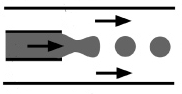
\includegraphics[height=4cm]{1_antecedentes/co_flow.jpg}}
    \subfloat[]{
     \label{subfig:cross_flow}
     \ref{subfig:cross_flow}
      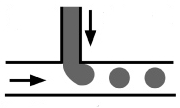
\includegraphics[height=4cm]{1_antecedentes/cross_flow.jpg}}
      
    \subfloat[]{
     \label{subfig:flow_focusing}
     \ref{subfig:flow_focusing}
      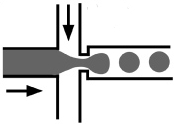
\includegraphics[height=5cm]{1_antecedentes/flow_focusing.jpg}}
      
  \end{center}
  \hspace{-7mm}
  \caption{\small Representación de las tres grandes geometrías microfluidicas usadas con mayor frecuencia en los chips de generación de \gotas. La geometría de las figuras reciben los nombres de \anglicismo{co-flow}
  %flujo conjunto
  (\ref{subfig:co_flow}); 
  \anglicismo{cross-flow}
  %flujo cruzado
  (\ref{subfig:cross_flow}), 
  % flujo de enfoque
  \anglicismo{flow focusing} (\ref{subfig:flow_focusing}). 
  En esta representación la fase dispersa se representa de color gris y la fase continua de color blanco. La dirección de los flujos se indica con las flechas. (Fuente: \url{http://cdn.iopscience.com/images/0022-3727/46/11/114002/Full/jphysd440265f01_online.jpg})
  }
  \label{fig:geometria_chips}
\end{figure}

% cross-flow, co-flow and flow-focusing geometries

En términos generales se distinguen tres grandes grupos llamados \anglicismo{co-flow} (flujo conjunto), \anglicismo{cross-flow} (flujo cruzado) y \anglicismo{low focusing} (flujo de enfoque) \citep{article:pingan}. Estos grupos también pueden clasificarse a su vez en dos tipos: simetría axial en 3D y planar cuasi-2D. Los dispositivos representados en la Figura~\ref{fig:geometria_chips} son todos de tipo planar cuasi-2D. En estos casos se utilizan canales relativamente planos en todas partes, de modo que su función se puede entender bien en una vista bidimensional.

En los dispositivos de \anglicismo{co-flow}, la fase dispersa y la fase continua convergen de forma paralela como puede verse en la Figura~\ref{subfig:co_flow}. El proceso físico implicado en la formación de las gotas está relacionado con la inestabilidad de Plateau-Rayleigh. Básicamente lo que ocurre es que las gotas se forman debido a que su forma esférica supone una mínimo en la superficie respecto a un volumen dado y esa disminución de la superficie supone un mínimo de energía; el mínimo de energía implica una forma estable. Estas gotas se forman de forma parecida a como lo hacen las gotas que caen de un grifo.

En los dispositivos de tipo \anglicismo{cross-flow}, las dos fases entran en contacto formando un ángulo. Un caso típico es la unión en T que se muestra en la Figura~\ref{subfig:cross_flow}. La fase dispersa, al encontrarse con la fase continua, la interrumpe y esta última presiona hasta que secciona un trozo de la fase dispersa de forma parecida a como haría una cizalla.


%Los otros emplean variaciones de confinamiento de canal para facilitar o impulsar la generación de gotitas, como la emulsificación por etapas, la emulsificación por microcanales y la emulsificación por membrana.
%( de forma general)

%%%file:///home/solorzaj/Documentos/Master/TFM/k_tfm_zhu2016.pdf(3.3 Flow-focusing)
%Los dispositivos microfluídicos de enfoque de flujo también pueden clasificarse a su vez en dos tipos: simetría axial en 3D y planar cuasi-2D. Los dispositivos que se han usado en nuestros experimentos siempre han sido de este último típo, planar cuasi-2D.
%Más tarde, en 2003, Anna et al. 63 por primera vez, tradujo la geometría de enfoque del flujo planar (Fig. 2c, ii) en un líquido- Sistema microfluídico líquido. En comparación con los dispositivos de enfoque de flujo planar, los dispositivos de enfoque de flujo asimétricos en 3D evitan problemas como la humectación de las paredes de los canales por la fase dispersa, produciendo gotitas monodispersas (CV). <5\%) con mayores rendimientos.

%Una rama de los dispositivos microfluídicos de enfoque de flujo 3D es el dispositivo microcapilar 55 (Fig. 2c, iii), donde los fluidos continuos y dispersos se suministran al dispositivo en direcciones opuestas y se encuentran en la entrada del orificio estrecho, luego se enfocan hacia abajo El orificio y la generación de gotitas uniformes. En combinación con la geometría de flujo conjunto, el dispositivo microcapilar (Fig. 2c, iv) puede generar Emulsiones múltiples monodispersas en un solo paso.


% file:///home/solorzaj/Documentos/Master/TFM/b_droplet_based_microfluidics_seemann2011.pdf (4.3.2. Co-flow/flow focusing)
Por último tenemos el caso llamado \anglicismo{flow focusing} (ver Figura~\ref{subfig:flow_focusing}). Esta es la geometría del chip  que usamos en nuestro dispositivo experimental. Su principio de funcionamiento es parecido al anterior. Cuando la fase dispersa (gris) bloquea la entrada estrecha en el canal a la derecha, la fase continua (blanco), entrando desde arriba y desde abajo en la figura, comienza a empujar hasta que las dos interfaces líquidas se unen y se forma la gota.

\subsubsection{Material para la fabricación del dispositivo.}\label{sec:antecedentes:materiales_chip}
%file:///home/solorzaj/Documentos/Master/TFM/b_droplet_based_microfluidics_seemann2011.pdf (standard device fabrication technique in science and research)

El material más utilizado para la fabricación de dispositivos microfluídicos actualmente es polidimetilsiloxano (PDMS). Las principales razones para ello son que tiene unas características físico-químicas generalmente deseables para la fabricación de los dispositivos utilizados en microfluídrica y microscopía y el proceso de fabricación sencillo, rápido y rentable utilizando la técnica llamada \anglicismo{softlithography}(litografía blanda).

El PDMS es un compuesto que pertenece al grupo de los organosilicatos poliméricos que comúnmente se conocen como siliconas. Su fórmula química para PDMS es $\mathrm{{CH}_{3} {[Si {({CH}_{3})}_{2} O]}_{n} Si {({CH}_{3})}_{3}}$.
%file:///home/solorzaj/Documentos/Master/TFM/2016_Book_MicrosystemsForPharmatechnolog.pdf (2.3.1 Polydimethylsiloxane) 
A temperatura ambiente, el PDMS es líquido y se puede convertir en elastómeros sólidos mediante un proceso llamado reticulación. El kit \comillas{Sylgard 184} disponible en el mercado de Dow Corning Inc. consiste en una base y un agente curante mezclado en una proporción de masa de 10:1. De acuerdo al módulo de Young del elastómero, si esta proporción aumenta, es el módulo disminuye. De esta forma podemos controlar la elasticidad final del polímero. La polimerización se realiza mediante una reacción de hidrosililación, donde los grupos vinilo $\mathrm{({CH}_{2}={CH}^{-})}$ de los oligómeros de siloxano forman enlaces covalentes con los grupos hidrosilano (SiH) del agente de curado. La reacción de reticulación se cataliza por un catalizador de platino contenido en el agente de curado y tiene lugar a temperatura ambiente, pero puede acelerarse aumentando la temperatura \citep{book:andreas}.

Como características deseables cabe destacar que tiene una buena estabilidad química, no es inflamable, no es tóxico y es biocompatible. Es permeable a los gases no polares como el $\mathrm{O}_{2}$ o el $\mathrm{CO}_{2}$ y no es hidroscópico. Es duradero y tiene una buena estabilidad térmica (soporta temperaturas de hasta 186~\celsius\ en el aire), una rigidez dieléctrica de 21 kV$\mathrm{{mm}^{-1}}$. Ópticamente es isótropo, homogéneo y transparente hasta los 300 nm.
Además presenta la gran ventaja de que se puede unir a sí mismo y a una serie de otros materiales (al vidrio por ejemplo) covalentemente después del tratamiento con plasma de aire.

A todas estas ventajas hay que sumar otras tantas características que generalmente no son deseables. Durante el curado su volumen se reduce aproximadamente un 1\% y puede hincharse en presencia de algunos solventes orgánicos como el tolueno y el hexano. Además puede absorber pequeñas moléculas hidrófobas y proteínas. 
%file:///home/solorzaj/Documentos/Master/TFM/b_droplet_based_microfluidics_seemann2011.pdf (Alternative device material)
En los casos en los que el PDMS no resulta adecuado, las alternativas suelen ser resinas a base de tioleno, tales como NOA81 o NOA83H \citep{article:ralf}.

\subsubsection{Fase dispersa y fase continua.}\label{sec:antecedentes:fases}
La fase dispersa contiene los reactivos que van a ser encapsulados juntos. En la mayor parte de las aplicaciones de secuenciación en gotas, esta fase incluye las células, los agentes de lisis y los reactivos necesarios para generar las librerías de secuenciación. En nuestro caso, en el que intentaremos separar los procesos de lisis y generación de la librería, nuestras gotas contendrán únicamente las células y agarosa. Esta agarosa, al enfriarse, atrapara a las células diana en su interior.   

La fase continua, debe ser un liquido inmiscible con el anterior. Esta fase suele ser un aceite al que se le han añadido surfactantes que impiden que las gotas se unan y formen de nuevo una fase continua.  Es importante elegir un sistema de aceite/surfactante adecuado en función las características de la fase dispersa y del material con el que está hecho el chip de encapsulado.
Para el caso de fase dispersa con base acuosa y dispositivos de PDMS sin recubrimientos de superficie especiales, se suelen usar aceites fluorados como FC40, FC70 (DuPont).
%La hinchazón se puede evitar o reducir usando otros materiales del dispositivo o aplicando recubrimientos de superficie (como se explicó anteriormente en la sección 2) o eligiendo otra fase portadora. 
%Como se comentó anteriormente, el PDMS puede absorber moleculas hidrofobas. Para evitar los efectos de hinchamiento en dispositivos PDMS a menudo se emplean aceites fluorados como FC40, FC70 (DuPont) o perfluorodecalina como una fase portadora que requiere surfactantes fluorados tales como pentadecaflouoro-1-octanol o poliéter perfluorado con Krytox, DuPont).
A pesar de que los aceites fluorados no hinchan notablemente el PDMS, estos pueden difundirse a través del PDMS y lixiviar los compuestos del material de PDMS. La difusividad de gas y vapor a través de algunos aceites, en particular a través de aceites fluorados, bastante grande y puede ser una desventaja para algunas aplicaciones, ya que esto puede suponer contaminaciones cruzadas y la pérdida de algunas sustancias.
Esta propiedad también se puede usar para estimular un intercambio controlado de iones seleccionados entre gotas o para proporcionar suministro de oxígeno para las células encapsuladas en gotas acuosas. La biocompatibilidad se puede lograr utilizando aceites fluorados junto con un surfactante combinado con un poliéter perfluorado y polietilenglicol para estabilizar gotitas acuosas. En nuestro caso, la difusividad de los gases y la biocompatibilidad de las gotas de agarosa y la fase continua no resultan demasiado importantes \citep{article:ralf}.